% ======================================================================
% col: 20

\chapter{Introduzione}
\label{chap:intro}

% Di seguito si descrivono le tecnologie usate e i concetti base che è necessario conoscere.

\section{F1TENTH}
F1TENTH è una community internazionale di ricercatori, ingegneri e appassionati di sistemi autonomi
che organizza competizioni di corsa di veicoli-robot con la peculiare caratteristica
di essere \textit{un decimo} di quelle di F1, da cui il nome.
\begin{wrapfigure}{r}{0.3\textwidth}
	\centering
	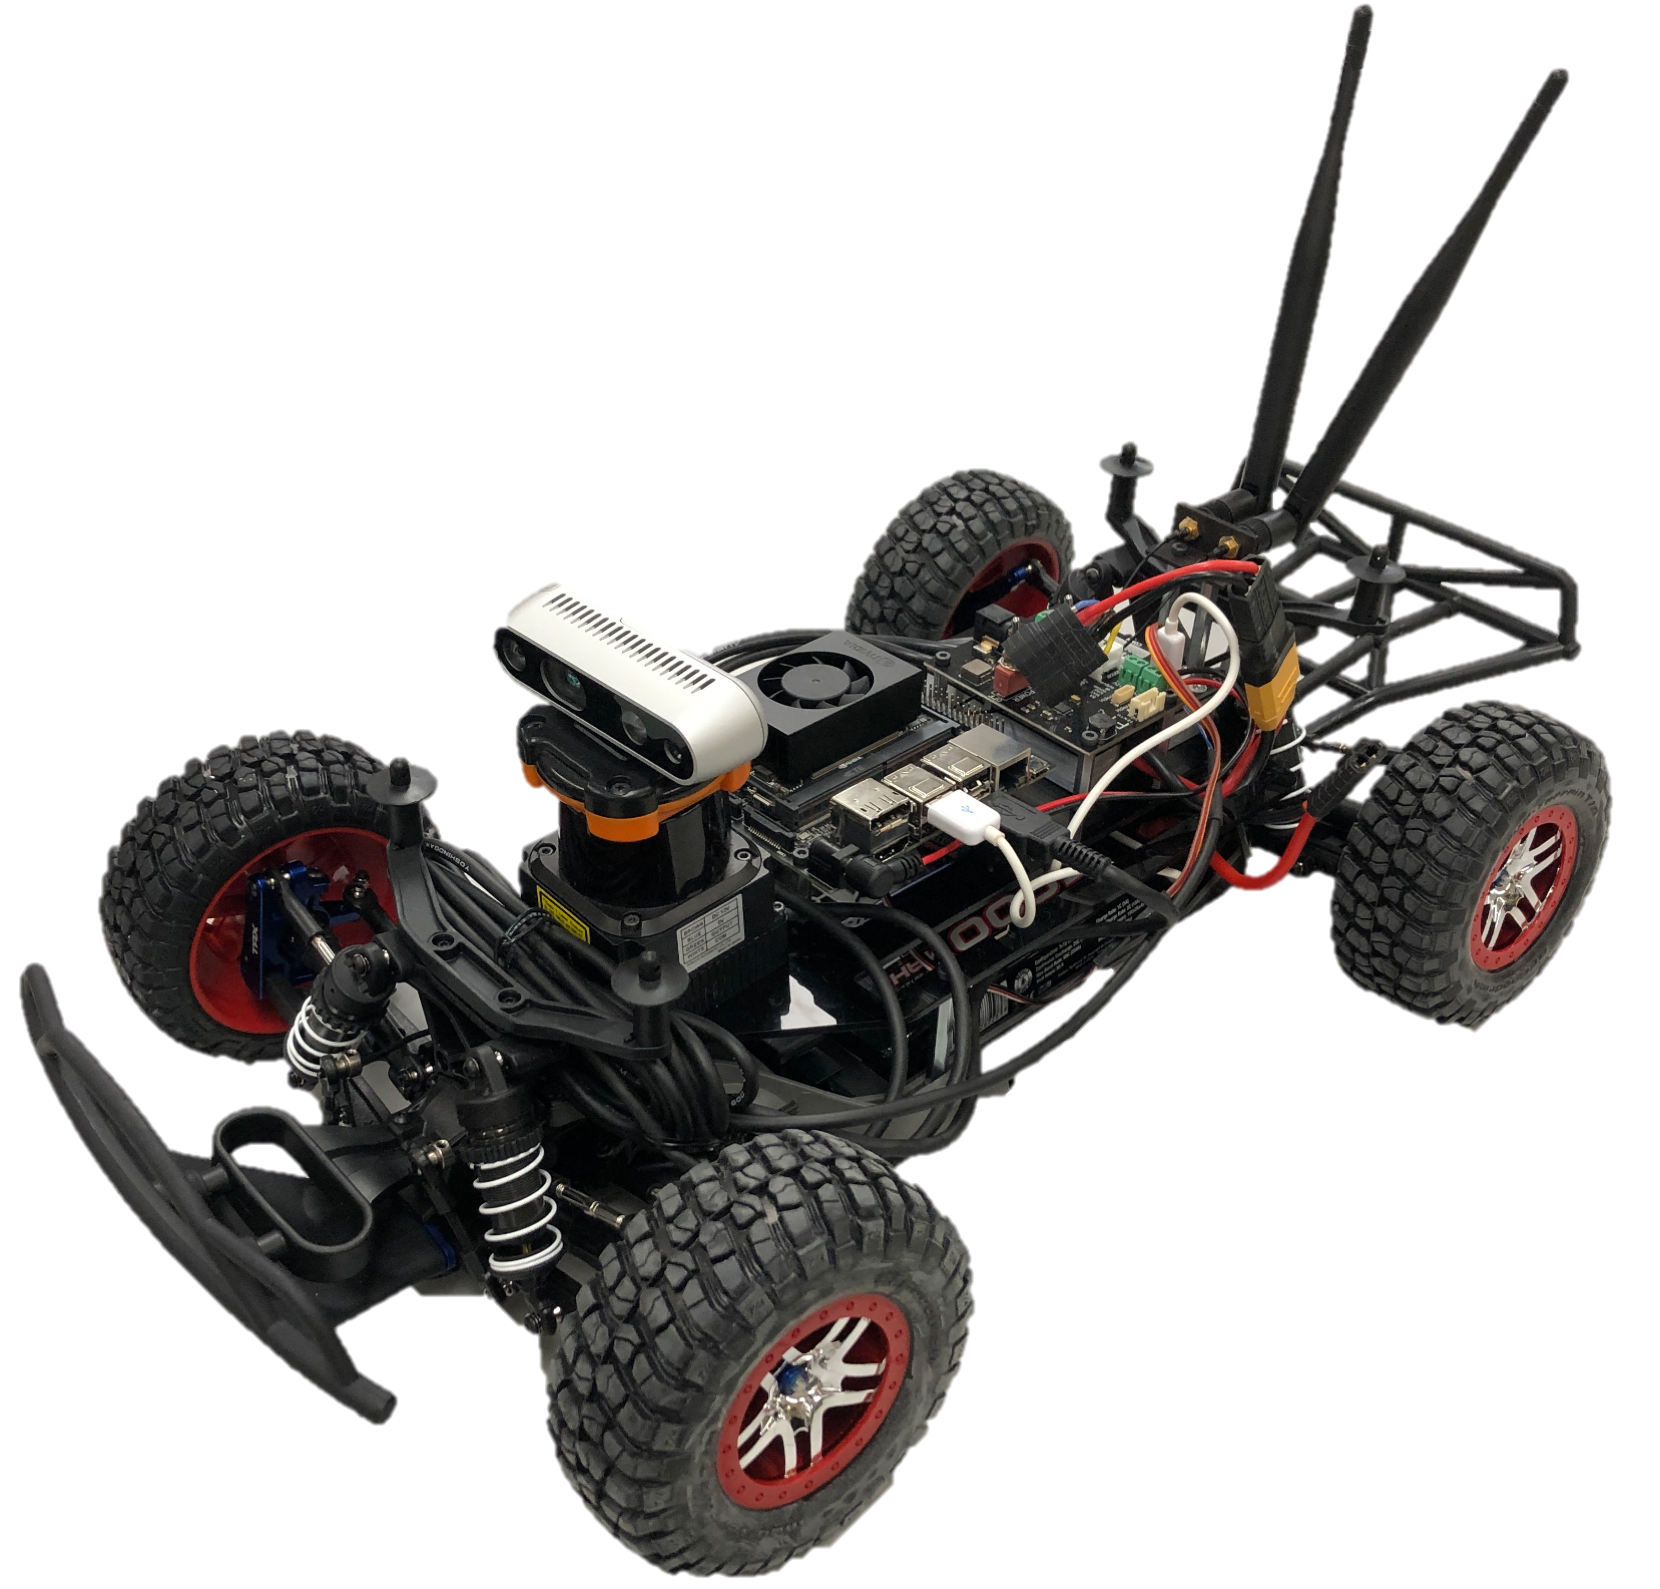
\includegraphics[width=0.2\textwidth]{f1tenth-car.png}
	{\footnotesize \\Robot di F1TENTH \cite{overview}}
\end{wrapfigure}
Oltre a questo, promuove la ricerca nell'ambito della guida autonoma
e altri campi tra cui reinforcement learning, sistemi di comunicazione e robotica;
offre, inoltre, una infrastruttura per costruire l'auto da corsa
e sviluppare il software necessario per farla gareggiare. \cite{f1tenth-web}

La community è stata fondata all'Università della Pennsylvania nel 2016 ma ha iniziato rapidamente
collaborazioni con altre istituzioni e università in tutto il mondo~--~in Italia, alla data di stesura, solo
con l'Università degli Studi di Modena e Reggio Emilia. \cite{f1tenth-about}

\paragraph{Moduli}
Il percorso di apprendimento, che ha materiale per un semestre circa,
% https://f1tenth.org/learn.html},
raggruppa le lezioni in moduli e li integra con altrettanti laboratori guidati
dove poter applicare le nozioni e algoritmi imparati.
\newpage % da rivedere per non spaccare la lista in più pagine
\noindent I moduli si raggruppano per tipologia di argomento trattato \cite{f1learn}:
\begin{itemize}
	\item \textit{Modulo A} -- Introduzione a \hyperref[sec:ros]{ROS} e 
		all'ambiente simulatore di \hyperref[par:gym]{F1TENTH~gym};
	\item \textit{Modulo B} -- Metodi reattivi e dinamiche del veicolo: \\
	      Descrive la modellazione delle dinamiche fisiche di un veicolo e presenta algoritmi di navigazione
	      reattivi come \textit{PID Control} e \textit{Wall following};
	\item \textit{Modulo C} -- Mapping \& Localization: SLAM e Particle Filter:\\
	      Introduzione alla stima dello stato, filtro di Bayes e varianti come Particle filter, uso di
	      algoritmi basati su filtri per la localizzazione del robot data una mappa, algoritmi localizzazione e
	      di modellazione dell'ambiente come SLAM;
	\item \textit{Modulo D} -- Planning \& Control: Pure Pursuit e RRT:\\
	      Descrizione dello stack di pianificazione e controllo di un veicolo autonomo, algoritmo di
	      \textit{path tracking} Pure Pursuit basato sulla dinamica del veicolo, introduzione ai
	      \textit{local planner} e algoritmi come RRT, spline e clotoidi per descrivere un percorso,
	      State lattice planner, Graph based planner;
	\item \textit{Modulo E} -- Vision:\\
	      Introduzione a Classical Perception, differenze hardware, stima della distanza, visual SLAM,
	      percezione basata su ML, object detection;
	\item \textit{Modulo F} -- Argomenti speciali: \textbf{\textit{Raceline Optimization}}, MPC:\\
	      Ottimizzazione del percorso di gara, Model Predictive Control e Moral Decision Making;
	\item \textit{Modulo G} -- Applicazione delle tecnologie descritte su gara simulata;
\end{itemize}

\noindent Ai fini dell'obiettivo di questa tesi si è preferito non approfondire il Modulo E,
in quanto si rendeva necessario l'uso fisico di hardware di cui non si aveva accesso,
ovvero l'auto e soprattutto sensori di visione come telecamere e LiDAR.

\paragraph{F1TENTH gym}
\label{par:gym}
% https://docs.google.com/presentation/d/1zfzzjVTbXNIZ75BFtGEwQBJRHlY95VKkFQjJhYfznpI/edit#slide=id.g1cca33b1c19_0_3213
La community sviluppa e mantiene un simulatore open-source specifico per F1TENTH \cite{f1tenth-gym}
in modo da poter sviluppare e testare comodamente
senza l'uso di hardware specifico definito per la costruzione del robot.\\
Il simulatore permette di definire la dinamica del veicolo in modo tale da avere una simulazione
più reale possibile. 


% ================== Autonomous Driving Pipeline =======================
\section{Autonomous Driving Pipeline}
\label{sec:pipeline}
Un progetto ben strutturato è più efficiente da mantenere e ha maggiori probabilità
di funzionare correttamente: ciò si applica anche in questo caso.\\
Un progetto complesso come quello dei veicoli autonomi deve essere suddiviso in sotto-problemi
più specifici e in modo tale che uniti insieme risultino nella soluzione del problema.

\bigskip
\noindent Il \emph{software} per i veicoli autonomi segue un \textit{ciclo} di operazioni
in cui il prodotto di una fase è input della successiva; si identificano in ordine tre fasi:
\begin{enumerate}
\item \textbf{Perception} -- Attraverso sensori ottici e radar si \emph{percepisce} il mondo attorno a sè,
	  ci si localizza nella mappa e si identificano eventuali ostacoli o rivali;
\item \textbf{Planning} -- Stando ai dati generati nella fase precedente,
	  si determinano quali saranno le \emph{mosse future} seguendo delle policy prescritte;
\item \textbf{Control} -- Si generano dei comandi di sterzata e di velocità per attuare le scelte
	  determinate nella fase precedente.
\end{enumerate}

L'input per la prima fase (\textit{Perception}) e l'ouput dell'ultima (\textit{Control})
è direttamente l'hardware: dunque nella prima sono i sensori ottici e radar, come citato precedentemente,
mentre nella seconda sono gli attuatori per i controllo della velocità e angolo delle ruote.

Il risultato che si vuole ottenere, quindi, è quello di una sequenza di comandi di sterzata e
accelerazione in un contesto, quello delle corse, che richiede una certa velocità di esecuzione per poter
essere il più reattivi possibile, per questo motivo è preferibile eseguire il ciclo tra le 20 e 50 volte
al secondo. Una rappresentazione grafica della pipeline intera si trova alla figura~\ref{fig:av-pipeline}.

\begin{figure}[H]
\centering
\caption{Pipeline per i veicolo autonomi \cite{overview}}
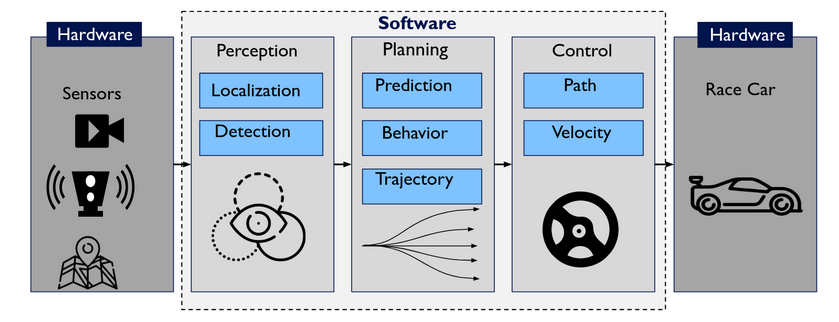
\includegraphics[width=\textwidth]{AV-pipeline.png}
\label{fig:av-pipeline}
\end{figure}

Di seguito si analizzano più nel dettaglio le fasi sopra citate.
\subsection{Perception} 
La prima fase ha il compito di \textit{analizzare} i dati prodotti da diversi tipi di sensori come quelli
ottici, laser e IMU (Inertial Measurment Unit) e ha come obiettivi quelli di: \cite{betz2022autonomous}
\begin{itemize}
	\item determinare l'ambiente statico, chiamato anche \textit{mappa}, che in questo contesto
	      rappresenta i confini del tracciato in cui il robot gareggia;
	\item eventuali ostacoli o altri robot rivali, che quindi compongono la
	      parte dinamica; 
	\item \textit{localizzarsi} all'interno della mappa, ovvero
	      determinare posizione e orientamento del robot rispetto alla mappa.
\end{itemize}
In questa fase, quindi, si ritrovano algoritmi di object detection -- di cui però non è stato argomento
di studio per questa tesi -- algoritmi di mapping e localization, come Particle Filter e SLAM
(\textit{S}imultaneous \textit{L}ocalization \textit{A}nd \textit{M}apping).

\paragraph{Localization}
% https://docs.google.com/presentation/d/1EAzm9A7FbAZFmA8l3ZNb2qjY_GqrLP0r-0uYwL0lLfs/edit#slide=id.g11505ea6fbe_0_901
Sebbene possano essere sfruttate tecnologie come il GPS, la ricerca nelle corse autonome si concentra
maggiormente su una soluzione che richieda solo l'uso di sensori ottici, laser e odometria.
\cite{betz2022autonomous} Per effettuare la localizzazione del robot è necessario avere un modello della
mappa.

Una prima soluzione potrebbe essere quella di partire da una posizione nota e di calcolare la posizione
successiva integrando le misurazioni dei vari sensori e l'odometria delle ruote: questa tecnica viene
chiamata \textit{Dead Reckoning} e, sebbene possa funzionare correttamente in un simulatore, nella realtà
le misurazioni dei sensori contengono del rumore e l'odometria delle ruote generalmente non ha la
precisione richiesta per via di un possibile slittamento delle ruote stesse: tutto ciò, quindi, introduce
nei calcoli degli \textit{errori} che si accumulano col tempo, portando a risultati errati.

La soluzione è quella di rendere più robusti i calcoli tenendo conto del rumore dell'odometria e dei
sensori e compensare alla mancanza di informazioni riguardo la posizione iniziale. Gli algoritmi
modellano questo aspetto usando il \textit{calcolo delle probabilità}. I principali sono: il già citato
Particle Filter, noto anche come AMCL (Adaptive Monte Carlo Localization) e principale algoritmo di
localization usato nello studio di questa tesi e nei laboratori, filtro di Bayes e derivati come Kalman
filter.

\paragraph{SLAM}
\label{par:slam}
SLAM è una tecnica che consente ai robot di eseguire simultaneamente la localizzazione e il mapping
di un ambiente sconosciuto. Siccome i problemi di mapping e localization necessitano l'uno dell'altro
per per poter essere risolti, è necessario risolverli contemporaneamente se non si hanno dati
nè sull'ambiente nè sulla posizione del robot.\\
Ad alto livello, l'algoritmo segue questi passaggi:
% NOTE: da rivedere/rimuovere nel caso
\begin{enumerate}
	\item \textit{prima scansione}: si usa la prima scansione come mappa iniziale;
	\item \textit{cambio della posizione}: il robot si muove di una certa quantità in un piccolo
	      lasso di tempo, si registra quindi una nuova scansione della mappa;
	\item \textit{stima della posizione}: la nuova scansione viene correlata con la mappa per
	      stimare il cambiamento di posizione;
	\item \textit{aggiornamento della mappa}: si integra la nuova scansione nella costruzione della mappa
	      sovrapponendo le misurazioni.
\end{enumerate}

\subsection{Planning}
La fase di Planning è stata argomento di studio approfondito di questa tesi, perciò verrà descritta
completamente nel Capitolo~\ref{chap:plan} a pag.~\pageref{chap:plan}.

\subsection{Control}
La terza fase prevede di attuare le decisioni calcolate nella fase di planning: deve quindi generare, in
questo contesto, dei controlli di accelerazione e angolazione delle ruote. In realtà questa fase rientra
in un più vasto e più generale campo di studi: l'\textit{ingegneria del controllo} (o dell'automazione).\\
I principali problemi che bisogna affrontare in questa fase sono:
\begin{itemize}
	\setlength\itemsep{0em}
	\item[$-$] come seguire una traiettoria data?
	\item[$-$] come compensare gli errori degli attuatori?
	\item[$-$] come guidare il più velocemente possibile?
\end{itemize}
Si fanno distinzione di due tipologie di algoritmi di controllo: gli \textit{open-loop} e
\textit{closed-loop}, chiamati anche feedback. In questo contesto, la differenza tra i due è che la
seconda tipologia di algoritmi riceve in input, appunto in \textit{feedback}, anche lo stato corrente del
veicolo rispetto agli output di controllo generati precedentemente; in questo modo è possibile calcolare
l'errore tra il comando calcolato e l'effettivo risultato dell'applicazione di quel comando dagli
attuatori, così da poterlo compensare al prossimo comando inviato.

\paragraph{PID Controller} \cite{lection04, pid-wiki}
L'algoritmo più conosciuto, specialmente per la sua semplicità, è il \textit{PID Controller} che viene
usato ampiamente in tutta l'industria dell'ingegneria del controllo, non solo in questo contesto.\\
PID è un acronimo che sta per \textbf{P}roportional-\textbf{I}ntegral-\textbf{D}erivative e questo
suggerisce che l'ouput è calcolato secondo tre parametri. Si tratta di un algoritmo closed-loop.

Con \textbf{proporzionale} si intende che il comando generato deve essere proporzionale all'errore tra lo
stato corrente del robot e lo stato desiderato.
Siccome ci si vuole che l'errore diminuisca col tempo, con \textbf{derivativo} si intende che si applica
una correzione all'ouput che è proporzionale alla velocità con cui l’errore si riduce.
Infine, con \textbf{integrale} si applica un'ulteriore correzione calcolata sia dalla magnitudine
dell'errore sia dalla sua durata nel tempo, ovvero si correggono gli errori accumulati nel tempo che
avrebbero dovuto essere corretti prima.

\paragraph{Pure Pursuit} \cite{lection10}
Un'altro algoritmo closed-loop più specifico per le corse di robot è Pure Pursuit. In questo caso, il
problema richiedere una sequenza di waypoint, ovvero punti nella mappa che formano un \textit{tracciato},
che il robot deve seguire. L'algoritmo tiene conto della dinamica del veicolo, che in questo caso è
\textit{non-holonomic}, quindi calcola l'arco che congiunge il robot e il primo waypoint che si trova ad
una distanza prefissata, il lookahead, dalla macchina.\\
Questo è stato il principale algoritmo usato nei laboratori e nello studio della tesi, seppur con qualche
modifica migliorativa.


% ================== ROS 2 ================================
\section{ROS2 }
\label{sec:ros}
% cit: https://docs.ros.org/en/humble/Citations.html
% https://www.ros.org/blog/ecosystem/
% https://www.ros.org/blog/why-ros/
% https://www.ros.org/blog/getting-started/#
% https://index.ros.org/packages/
% http://design.ros2.org/articles/changes.html ros1 vs ros2
ROS è un acronimo che sta per \textbf{R}obot \textbf{O}perating \textbf{S}ystem e,
sebbene il nome possa trarre in inganno, non è un sistema operativo nel senso tradizionale,
bensì si presenta come un mediatore -- un \textbf{middleware} -- tra l'applicazione robot
e l'hardware del robot, ma non sostituisce il sistema operativo sottostante. \cite{ros-ecosystem}\cite{scirobotics}

Viene usato da tutta l'industria della robotica per via della sua alta modularità:
dalla ricerca all'insegnamento, da progetti di un gruppo di persone a progetti più importanti
di grosse aziende. ROS fornisce i \textit{building blocks} da usare così da facilitare e velocizzare
la realizzazione dell'applicativo e fornisce un metodo di comunicazione efficiente tra le varie componenti.

Il progetto è \href{https://github.com/ros}{\textit{open-source}} ed ha una grossa community di
sviluppatori e ricercatori internazionale che lo mantiene e distribuisce pacchetti integrativi per
diverse funzionalità come driver per i sensori e attuatori, algoritmi noti, compatibilità con altri
programmi, visualizzazioni in tempo reale e tante altre funzioni di utilità. In questo senso, ROS si
presenta più simile a un \textit{SDK} (Software Development Kit) accompagnato da una serie di tools,
principalmente a linea di comando.

ROS viene rilasciato con la stessa filosofia delle \textit{distro linux}, con più distribuzioni mantenute
nello stesso tempo. Va notato che le differenze tra ROS e ROS2 sono profonde differenze
di design e aggiornamento delle tecnologie come, per esempio, l'aggiornamento dei linguaggi supportati,
il sistema di build e importanti modifiche alla gestione dei \hyperref[ros:msgs]{messaggi} e servizi. \cite{ros-diff}
Attualmente, ROS e ROS2 supportano due linguaggi: C++ e Python. In questa tesi è stato usato Python.
Durante lo studio di questa tesi è stato usato ROS2, distribuzione
\href{https://docs.ros.org/en/humble/}{\textit{"Humble"}}, per necessità di compatibilità con alcuni
pacchetti.

\bigskip
\noindent ROS, fondamentalmente, fornisce un metodo di comunicazione tra le componenti dell'applicativo,
che vengono chiamati \hyperref[ros:nodes]{\textbf{\textit{Nodi}}}, attraverso diversi sistemi tra cui i
\hyperref[ros:topics]{\textbf{\textit{Topic}}}, i \hyperref[ros:srv-act]{\textit{Servizi} e le
\textit{Azioni}}. L'insieme dei nodi e dei loro collegamenti formano il \textit{ROS~Graph}, il grafo dei
nodi.

\medskip
\begin{figure}[h]
	\centering
	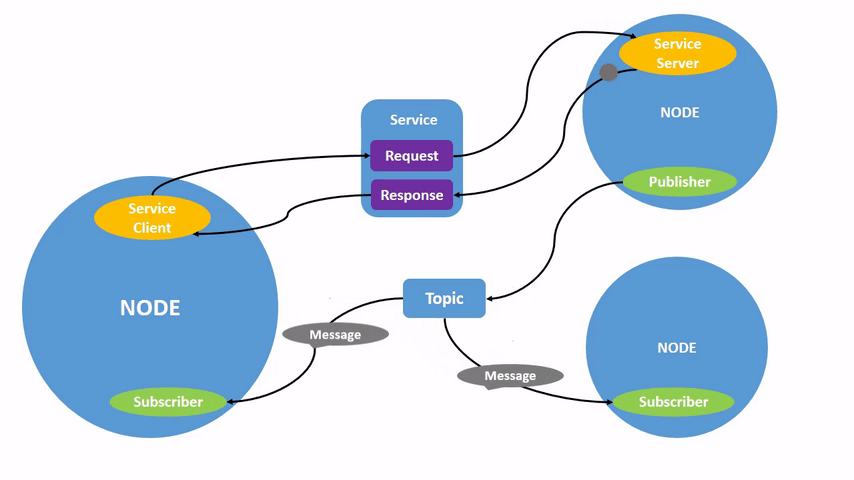
\includegraphics[width=1\textwidth]{ros-topic-srv.png}
	\caption{Esempio di ROS Graph \cite{lection01}}
	\label{fig:ros-topic-srv}
\end{figure}
\noindent Di seguito si analizzano le componenti principali di cui ROS è composto.
% https://docs.ros.org/en/iron/Concepts/Basic.html
\paragraph{Nodi \cite{undr-nodes, ros-nodes}} 
\label{ros:nodes}
% https://docs.ros.org/en/iron/Tutorials/Beginner-CLI-Tools/Understanding-ROS2-Nodes/Understanding-ROS2-Nodes.html
% https://docs.ros.org/en/iron/Concepts/Basic/About-Nodes.html
I nodi, \textit{Nodes} in inglese, sono l'unità computazionale che partecipa al ROS Graph;
idealmente, un nodo dovrebbe essere responsabile di un solo compito, logicamente separato
da altri altri, per esempio controllare le ruote, processare i dati grezzi derivati dalle misurazioni
dei laser o implementare un algoritmo come Pure Pursuit.
Un completo sistema robotico comprende, quindi, un insieme di nodi che lavorano congiuntamente, spesso
contenuti nello stesso eseguibile.\\

\paragraph{Topic \cite{undr-topics, ros-topics}}
\label{ros:topics}
% https://docs.ros.org/en/iron/Concepts/Basic/About-Topics.html
% https://docs.ros.org/en/iron/Tutorials/Beginner-CLI-Tools/Understanding-ROS2-Topics/Understanding-ROS2-Topics.html
I topic sono il principale strumento con cui i nodi di un ROS Graph si \textit{scambiano dati}.
I topic sono entità \textbf{\textit{fortemente tipizzate}} che implementano
un pattern \textbf{\textit{publisher/subscriber}} di tipo \textit{anonimo}, ciò significa
che i nodi conoscono una interfaccia comune con cui scambiarsi messaggi ben definiti.\\
\textit{Anonimo} significa che chi invia o riceve dei messaggi da o verso un topic
non ha modo di identificare mittente o destinatario perché, in questo contesto, non ha una grossa rilevanza,
sebbene esistano comunque dei modi per scoprirlo; inoltre, ogni messaggio generato da un publisher
viene ricevuto da ogni subscriber, nell'idea che un nodo si sottoscriva a un topic solo se ne è
interessato; questo ha il vantaggio di una grossa flessibilità in termini di manuntenibilità.\\
I nodi possono \textit{pubblicare} e \textit{sottoscriversi} ad un numero arbitrario di topic
per inviare e ricevere dati da altri componenti del grafo: si può avere quindi una relazione uno a
uno, uno a molti, molti a uno e molti a molti.\\
I topic vengono identificati da una stringa univoca che ne rappresenta il nome.

\paragraph{Messaggi \cite{ros-message}}
\label{ros:msgs}
% https://docs.ros.org/en/iron/Concepts/Basic/About-Interfaces.html#messages
I messaggi sono l'\textit{interfaccia}, agnostica al linguaggio, con la quale i \hyperref[ros:nodes]{nodi}
comunicano tra di loro. Descrivono un tipo di dato strutturato \textbf{fortemente tipizzato} in un
file con estensione \verb|.msg|. Questo tipo di file contiene una lista di attributi definiti da
tipo dell'attributo, nome ed eventuale valore di default. Il tipo può essere un tipo base
(\verb|short|, \verb|double|, \verb|string|) o un tipo composto, ovvero un'altro tipo messaggio.

\paragraph{Parametri e Launch files \cite{ros-params, ros-launch}}
% https://docs.ros.org/en/humble/Concepts/Basic/About-Launch.html
% https://docs.ros.org/en/humble/Concepts/Basic/About-Parameters.html
É possibile parametrizzare i nodi in modo da configurarli sia all'avvio sia durante l'esecuzione
senza cambiare codice e ricompilarlo. I parametri consistono in una coppia chiave-valore ed una
opzionale descrizione, che può indicare eventuali vincoli di tipo e range di valori.\\
Spesso i parametri vengono inizializzati all'avvio del nodo attraverso quelli che vengono chiamati
\textit{launch file} usati col comando \verb|ros2 launch| e che quindi permettono di avere \textit{diverse
configurazioni dello stesso nodo} senza doverlo ricompilare. Un'altro caso d'uso è durante la fase di
tuning per alcuni algoritmi: se il contesto lo permette è possibile modificare online i valori dei
parametri (per esempio da CLI), a patto che venga gestito nel codice del nodo.
I launch file possono essere usati anche per avviare più nodi contemporaneamente, in modo da
automatizzare l'intero applicativo.

\paragraph{Services e Actions \cite{ros-services, ros-actions}}
\label{ros:srv-act}
% https://docs.ros.org/en/humble/Concepts/Basic/About-Actions.html
% https://docs.ros.org/en/humble/Concepts/Basic/About-Services.html
Altri due sistemi di comunicazioni fra \hyperref[ros:nodes]{nodi} sono i Servizi e le Azioni.
Questi sono sostanzialmente chiamate remote -- ovvero ad altri nodi -- a procedure seguendo il paradigma
client/server. La loro principale differenza è concettuale e si discrimina dalla velocità di esecuzione:
nei servizi, infatti, la risposta deve essere rapida, mentre nelle azioni ci si aspetta una esecuzione
più lunga, anche di minuti, e si ha la possibilità di cancellarla prima del suo termine.
Entrambi vengono definiti con strutture simili ai messaggi, con file di diversa estensione.

Per citare qualche esempio, nei servizi troviamo operazioni di trasformazioni di coordinate tra frame, mentre
nelle azioni operazioni di più alto livello come \textit{"raggiungi questo waypoint"}.


\bigskip

La figura \ref{fig:ros-topic-srv} rappresenta un ROS Graph comprendente tre nodi, un topic e un servizio;
al topic sono sottoscritti i nodi in basso e ricevono i messaggi prodotti dal nodo in alto a destra che
fa anche da server al servizio da cui riceve richieste dal nodo client.

\section{RViz}
\label{sec:rviz}
RViz (\textbf{R}os \textbf{Vi}suali\textbf{z}er) è il principale strumento di visualizzazione 3D per gli
applicativi ROS. Durante lo studio di questa tesi è stato usato per visualizzare la simulazione di
F1TENTH gym, il modello del robot, la mappa del circuito ed eventuali visualizzazioni dei vari algoritmi
in studio, per esempio i waypoint di goal per Pure Pursuit, l'albero dei punti random generati da RRT e i
waypoint che compongono la raceline ottima.\\
La figura \ref{fig:rviz-example} ne mostra un'esempio.

\begin{figure}[H]
	\centering
	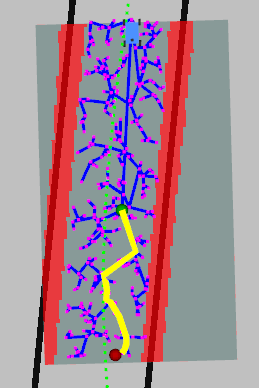
\includegraphics[width=0.4\textwidth, height=0.45\textheight, angle=90]{rrt.png}
	\caption{Esempio di caso d'uso di RViz per visualizzare l'algoritmo RRT}
	\label{fig:rviz-example}
\end{figure}
